\chapter{Zero knowledge}
\section{Crittografi mangiatori}
Ci sono 3 crittografi che cenano insieme, durante la loro cena discutono di tutto, ma essendo 
paranoici non possono far a meno di notare un personaggio misterioso che li osserva. Al momento 
del conto decidono di pagare ognuno la propria parte, ma il cameriere gli dice che il conto è
stato già pagato. I crittografi vogliono capire se il personaggio misterioso ha pagato il conto
o se è stato uno di loro, ma non vogliono rivelare il proprio contributo. Come possono fare?
\begin{figure}[H]
  \centering
  \begin{tikzpicture}
    % Filosofi
    \node[groom, female, minimum size=1cm, label=below:{Alice}] (A) at (0,0) {};
    \node[groom, mirrored, minimum size=1cm, label=below:{Bob}] (B) at (5,0) {};
    \node[groom, minimum size=1cm, label=below:{Charlie}] (C) at (2.5,4) {};
    % Personaggio oscuro 
    \node[criminal, minimum size=1cm, label=below:{David}] (D) at (-5, 2.5) {};
    % Nodi
    \draw[->] (A) -- (B) node[midway, below] {$C_2$};
    \draw[->] (B) -- (C) node[midway, right] {$C_3$};
    \draw[->] (C) -- (A) node[midway, left] {$C_1$};
  \end{tikzpicture}
  \caption{Crittografi mangiatori}
\end{figure}
L'idea è quella di utilizzare un protocollo di \textbf{zero knowledge}, ovvero un protocollo che
permette di dimostrare di conoscere una certa informazione senza rivelarla. Ognuno di loro 
nasconde un bit $b_i$ che indica se ha pagato o meno il conto, il bit varrà $1$ se ha pagato e $0$
altrimenti. 
Ovviamente è chiaro che se il risultato di tutti i bit è $0$ allora nessuno ha pagato, se invece
il risultato è $1$ allora ogni crittografo sa che almeno uno di loro ha pagato, ma non sa chi. Possiamo vedere 
questo calcolo come il calcolo di una funzione $f$ che prende in input i bit $b_i$ e restituisce
$1$ se almeno uno di loro ha pagato, $0$ altrimenti, partendo dall'assunzione che i partecipanti siano
onesti.

Ognuno di loro lancia una propria moneta a destra, ed ogni crittografo vede il risultato della
moneta del crittografo alla sua sinistra e ovviamente sa il risultato della propria moneta.
A questo punto ogni crittografo calcola lo \texttt{XOR} delle due monete a cui ha accesso.
\[
  x_{mine} = C_{other} \oplus C_{mine}
\]
$x_i$ varrà $0$ se le monete sono uguali, $1$ altrimenti. Il crittografo che ha pagato il conto 
complementa il proprio $x$.
\[
  x_{mine} = \overline{x_{mine}}
\]
A questo punto notiamo che ogni singolo elemento viene considerato due volte, quindi il risultato
dello \texttt{XOR} di tutti gli $x$ sarà $0$ se nessuno ha pagato, $1$ altrimenti. 
Ogni crittografo sa quello che può sapere conoscendo il proprio bit e il risultato della funzione, 
quindi da questo protocollo ogni crittografo può apprendere solo ed esclusivamente ciò che si può apprendere 
dalla conoscenza del proprio argomento e dalla conoscenza del risultato della funzione.
Chiaramente l'agente che sa di essere il crittografo che ha pagato sa il risultato degli altri 
crittografi.
\subsection{Generalizzazione del protocollo}
Il protocollo può essere generalizzato a \(n\) crittografi, ognuno dei quali lancia una moneta e
ognuno di loro vede il risultato della moneta del crittografo alla sua sinistra, calcolando 
lo \texttt{XOR} tra le due monete. Ogni singola moneta viene conteggiata due volte, quindi
il risultato dello \texttt{XOR} di tutte le monete sarà \(0\) se nessuno ha pagato, \(1\) altrimenti
(\textit{eseguendo il complemento}), partendo dal presupposto che tutti i crittografi siano onesti.

\subsubsection{Agente esterno che incarica la trasmissione di un messaggio}
Supponiamo che qualcuno incarichi un crittografo di spedire un bit, ma non vuole comunicare 
chi è l'incaricato. Se il crittografo in questione si comporta come l'unico crittografo che 
può aver pagato, ha la capacità di spedire un bit senza che nessuno si accorga di chi è
stato l'incaricato.

\subsubsection{Agente interno che vuole spedire un messaggio}
Supponiamo che il tempo sia scandito da un clock. Al primo ciclo di clock, il crittografo \(i\) lancia la
moneta e la passa al crittografo alla sua destra. Al secondo ciclo di clock, il crittografo \(i\) calcola 
lo \texttt{XOR} tra la moneta che ha ricevuto e la moneta che ha lanciato. Il crittografo 
che vuole spedire il bit complementa il risultato, chi non vuole spedire il
bit lascia il risultato così com'è. 

Supponendo che il crittografo che vuole spedire il bit sia uno solo, riuscirà a spedire il bit
con successo.

Con questo protocollo però potrebbero esserci dei conflitti, ovvero potrebbe capitare che due
crittografi vogliano spedire un bit. I crittografi hanno modo di accorgersi di questo conflitto,
ogni crittografo riesce ad osservare il bit che è stato spedito nella rete, se il bit è diverso
da quello che ha spedito lui, allora sa che c'è stato un conflitto. In questo caso il crittografi 
che hanno spedito il bit e si accorgono gli il risultato non è andato a buon fine,
spediscono il bit ad un ciclo di clock casuale e riprovano.

\subsubsection{Agente interno che vuole spedire un messaggio ad un agente nascondendo il destinatario}
Per farlo basta utilizzare il metodo precedente criptando il messaggio con la chiave pubblica del
destinatario. In questo modo solo il destinatario potrà leggere il messaggio.

Il risultato è un sistema di comunicazione totalmente non tracciabile, non si sa chi ha spedito, 
non si sa il destinatario del messaggio e non si sa il contenuto del messaggio.
Il protocollo ha però dei difetti, è infatti molto dispendioso in termini di risorse, poiché 
tutti gli agenti devono essere sempre attivi ed è soggetto ad un attacco chiamato \textbf{denial of service},
se qualcuno vuole oscurare il canale può trasmettere
sequenze di bit casuali e nessuno saprà mai chi ha oscurato il canale.
\section{La caverna di Ali Baba}
L'idea si basa sul fatto che ci siano due agenti, Peggy e Victor. Peggy (\textit{prover}) vuole
dimostrare a Victor (\textit{verifier}) di conoscere una certa informazione, senza però rivelare
l'informazione stessa. Si vole inoltre che la conoscenza di Victor sull'informazione sia
\textbf{zero}, ovvero Victor non deve imparare nulla sull'informazione che Peggy vuole dimostrare
e che non sia nemmeno in grado di dimostrare di conoscere l'informazione a terzi.
\begin{figure}[H]
    \centering
    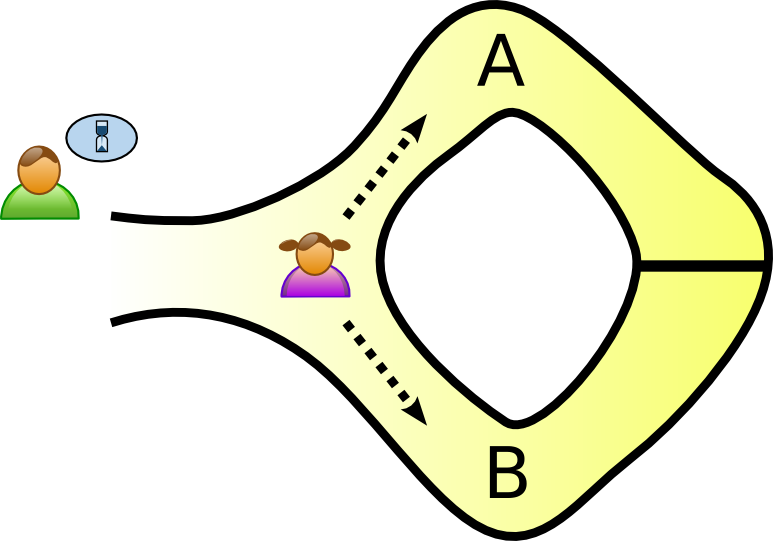
\includegraphics[width=0.35\textwidth]{img/zero_knowledge1.png}
    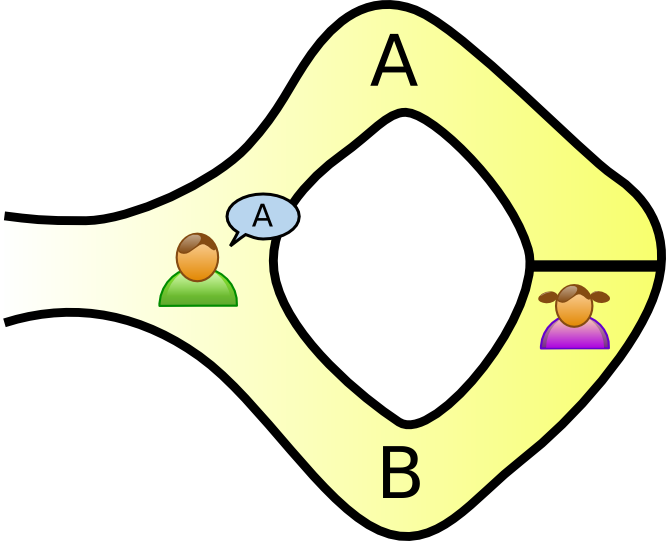
\includegraphics[width=0.3\textwidth]{img/zero_knowledge2.png}
    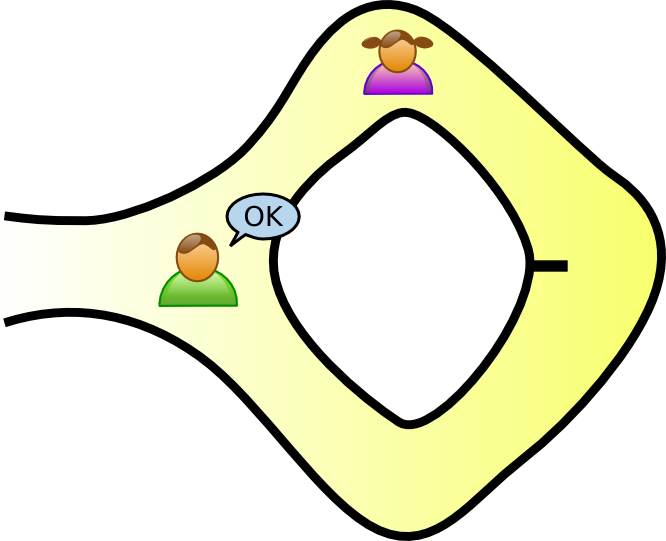
\includegraphics[width=0.3\textwidth]{img/zero_knowledge3.png}
    \caption{Peggy è in grado di dimostrare a Victor di conoscere l'informazione senza rivelarla,
    dimostrando di riuscire ad uscire dall'estremità corretta del labirinto.}
\end{figure}
Se Victor seguisse Peggy, potrebbe imparare l'informazione, quindi Peggy deve essere in grado di 
dimostrare di conoscere l'informazione senza che Victor possa impararla.
Se invece Victor andasse dalla parte opposta, non imparerebbe nulla, ma sarebbe in grado di 
dimostrare a terzi che Peggy conosce l'informazione, filmando l'apertura della porta.

Quello che si può fare è far scegliere da Peggy una delle due direzioni attraverso il lancio 
di una moneta, dopo che Peggy ha raggiunto la direzione decisa attraverso il lancio della moneta,
Victor raggiunge lo stesso punto di partenza di Peggy e lancia 
la moneta per decidere la direzione che Peggy deve prendere, Peggy deve quindi prendere la direzione
decisa da Victor. Se Peggy conosce l'informazione, riuscirà sempre a prendere la direzione decisa
da Victor, altrimenti con probabilità $\frac{1}{2}$ non sarà in grado di prendere la direzione
decisa da Victor.
Per abbassare la probabilità di errore, si può ripetere il protocollo più volte, in questo modo
se Peggy non conosce l'informazione, la probabilità di errore sarà $\frac{1}{2^k}$, dove $k$ è il
numero di volte che si ripete il protocollo.

Victor non sarà in grado di dimostrare a terzi che Peggy conosce l'informazione, poiché dall'ipotetico 
filmato che Victor potrebbe girare, non si capirebbe se i due hanno deciso la direzione in anticipo
o se Peggy conosce l'informazione, essendo che si vedrebbe solo la comunicazione della direzione da parte di Victor e
l'uscita di Peggy dalla direzione decisa da Victor.
\section{Classe \texttt{P} e \texttt{NP}}
Un problema decisionale $Q$ appartiene a \texttt{P} se esiste una macchina di Turing
deterministica (\textit{o equivalente}) che, in tempo polinomiale rispetto alla dimensione dell'input,
può risolvere il problema $Q$.

Un problema decisionale $Q$ appartiene a \texttt{NP} se e solo se esiste una macchina di Turing deterministica
(\textit{o equivalente}) che, in tempo polinomiale rispetto alla dimensione dell'input, può verificare soluzioni
proposte per ogni istanza $x$ di $Q$. 

\begin{theorem}
    Un linguaggio $\mathcal{L} \in \texttt{NP}$ se e solo se esiste un linguaggio 
    $\mathcal{L'}$ appartenente alla classe \texttt{P} tale che $\forall x \in \mathcal{L}$, esiste
    un certificato $y$ tale che $(x,y) \in \mathcal{L'}$.
\end{theorem}
In generale quindi dimostrare un teorema è più difficile che verificare che un teorema sia vero.
Se volessimo dimostrare che verificare non è più difficile che dimostrare potremmo farlo dando una 
potenza di calcolo limitata a chi verifica e una potenza di calcolo illimitata a chi dimostra.
\section{Interactive proof system}
Un \textbf{interactive proof system} è una coppia di algoritmi (\textit{macchine di Turing}) $(P,V)$, tali 
che $P$ ha potenza di calcolo illimitata e $V \in \texttt{PPT}$. $P$ e $V$ interagiscono scambiandosi 
messaggi e alla fine $V$ deve decidere se accettare o rifiutare l'input $x$.

Un linguaggio $\mathcal{L}$ ammette un \texttt{IPS} (\textit{Interactive Proof Space}) se
esistono due algoritmi, \(P\) e \(V\), tali che:

\[
\forall x \in \mathcal{L} \quad \mathcal{P}[(P,V) \text{ accetta } x] > \frac{2}{3}
\] 

\[
\forall x \notin \mathcal{L} \quad \forall P' \quad \mathcal{P}[(P',V) \text{ accetta } x] \leq \frac{1}{3}
\]

La classe di linguaggi che ammettono un \texttt{IPS} si chiama \texttt{IP}. Quindi, un linguaggio $\mathcal{L}$
appartiene a \texttt{IP} se ammette un \texttt{IPS}.

Inoltre, si ha l'inclusione di classi di complessità:

\[
\texttt{NP} \subseteq \texttt{IP}
\]

Il seguente teorema afferma l'equivalenza tra le classi di complessità
\texttt{IP} e \texttt{PSPACE}:

\begin{theorem}
    \texttt{IP} $=$ \texttt{PSPACE}
\end{theorem}
\begin{proof}
La dimostrazione di questa equivalenza coinvolge la costruzione di trasformazioni tra le classi \texttt{IP} e \texttt{PSPACE}
in entrambe le direzioni.
Per dimostrare \( \texttt{IP} \subseteq \texttt{PSPACE} \), si mostra che ogni problema risolvibile in modo interattivo
in tempo polinomiale ha anche una soluzione in spazio polinomiale.
La direzione opposta, \( \texttt{PSPACE} \subseteq \texttt{IP} \), richiede la costruzione di un protocollo interattivo
che possa simulare una macchina di Turing con spazio limitato e risolvere il problema in modo interattivo.
Pertanto, si conclude che \( \texttt{IP} \) e \( \texttt{PSPACE} \) sono equivalenti in termini di potenza computazionale.
\end{proof}
\subsection{Quadratic non-residuosity}
Tale problema è un problema appartenente alla classe di problemi \texttt{CO-NP}, perché verificare che un numero 
sia effettivamente un quadrato è un problema di \texttt{NP} e il certificato che mostra che un numero è un quadrato è
una delle due radici quadrate del numero.

Abbiamo un numero in $\mathbb{Z}_n^*$ che non è un quadrato e vogliamo costruire un interactive proof system
per dimostrare che non è un quadrato.

L'idea alla base è che se $x$ non è un quadrato, allora moltiplicando $x$ per un quadrato, il risultato non sarà un quadrato.

L'input del problema è la coppia $(n,x)$, e l'output accetta se $x$ è un non-residuo quadratico in $\mathbb{Z}_n^*$.
Victor manda a Peggy $w_1, w_2, \dots, w_l$ dove:
\[
  w_i = \begin{cases}
    z_i^2 & \text{con } z_i \in_R \mathbb{Z}_n^* \text{ se }b_i = 0 \text{ dove }b_i \in_R \{0,1\} \\
    x \cdot z_i^2 & \text{altrimenti}  
    \end{cases}
\]
Peggy invia a Victor la sequenza $c_1, c_2, \dots, c_l$ dove:
\[
  c_i = \begin{cases}
    0 & \text{se }w_i \text{ è un quadrato} \\
    1 & \text{altrimenti}
    \end{cases}
\]
Se $x$ non è un quadrato, allora $w_i$ è un quadrato se e solo se $b_i = 0$ e
non è un quadrato se e solo se $b_i = 1$. Victor accetta solo se $c_i = b_i$ per ogni $i$.
La se Peggy non conosce la soluzione, la probabilità che Victor accetti è $\frac{1}{2^l}$, 
mentre se la conosce la probabilità è $1$.
L'idea intuitiva è che la capacità di rispondere coincida con la conoscenza del segreto, in questo caso 
visto che nel mondo reale prover con potenza di calcolo illimitata non esistono, e visto 
che Peggy riesce a rispondere alle domande di Victor, allora Peggy conosce la fattorizzazione 
di $n$.
\subsection{Graph non-isomorphism}
Abbiamo due grafi $G_1$ e $G_2$ e vogliamo costruire un interactive proof system per dimostrare che non sono isomorfi,
$G_1 \not\simeq  G_2$. Ricordiamo che due grafi sono isomorfi se esiste una funzione biunivoca tra i vertici dei due
grafi che preserva gli archi.

\begin{figure}[H]
    \centering
        \begin{tikzpicture}
            \begin{scope}[every node/.style={circle,thick,draw}]
                \node (A) at (0,0) {A};
                \node (B) at (2.5,1) {B};
                \node (C) at (5,0) {C};
                \node (D) at (2.5,-3) {D};
                \node (E) at (0,2) {E};
                \node (F) at (5,2) {F} ;
            \end{scope}
            
            \begin{scope}[>={Stealth[black]},
                          every edge/.style={draw=black,very thick}]
                \path [-] (A) edge node {} (E);
                \path [-] (E) edge node {} (F);
                \path [-] (E) edge node {} (B);
                \path [-] (B) edge node {} (D);
                \path [-] (D) edge node {} (F);
                \path [-] (F) edge node {} (C);
                \path [-] (C) edge node {} (D);
                \path [-] (C) edge node {} (F);
                \path [-] (B) edge node {} (C); 
            \end{scope}
        \end{tikzpicture}
        \begin{tikzpicture}
            \begin{scope}[every node/.style={circle,thick,draw}]
                \node (A) at (0,0) {A};
                \node (B) at (0,3) {B};
                \node (C) at (2.5,4) {C};
                \node (D) at (2.5,1) {D};
                \node (E) at (2.5,-3) {E};
                \node (F) at (5,3) {F} ;
            \end{scope}
            
            \begin{scope}[>={Stealth[black]},
                          every edge/.style={draw=black,very thick}]
                \path [-] (A) edge node {} (B);
                \path [-] (B) edge node {} (C);
                \path [-] (D) edge node {} (C);
                \path [-] (D) edge node {} (E);
                \path [-] (D) edge node {} (F);
                \path [-] (C) edge node {} (F);
                \path [-] (E) edge node {} (F); 
                \path [-] (B) edge[bend right=60] node {} (E); 
            \end{scope}
        \end{tikzpicture}
    \caption{Esempio di due grafi isomorfi}
\end{figure}

\begin{tcolorbox}[title=Isomorfismo di grafi]
    Due grafi sono isomorfi, quando esiste un mapping biunivoco, che preserva 
    gli archi, tra i vertici dei due grafi.
\end{tcolorbox}

$V$ sceglie un grafo $G\in_R \{G_1, G_2\}$ e lo permuta casualmente in $G'$. $V$ invia $G'$ a $P$ e $P$ 
stabilisce se $G'$ è isomorfo a $G_1$ o $G_2$ e invia il risultato a $V$. $V$ accetta se $P$ indovina correttamente.

Il fatto che $P$ sia in grado di rispondere è dovuto al fatto che abbia potenza di calcolo illimitata e non 
è dovuto al fatto che vi siano informazioni trapdoor. 

Vorremo arrivare al punto che $V$ non impari nulla di più se non il non isomorfismo tra i grafi, poiché 
potrebbe esistere un $V$ che ha come obiettivo di sapere qualcosa in più, come ad esempio capire se $G_2$
è isomorfo a un altro grafo $G_3$. Per farlo parte dall'istanza di $G_1$ e $G_2$ per interagire con $P$, 
e la prima richiesta sarà proprio $G_3$. Usando quindi $P$ per risolvere problemi di cui non ha 
l'informazione. 

L'idea è che $V$ avrebbe potuto simulare l'interazione con $P$ senza interagire con $P$ stesso.
Se $P$ e $V$ interagiscono vengono prodotti una serie di messaggi, che in realtà sono una sequenza casuale,
perché $P$ e $V$ sono algoritmi stocastici, dove vengono effettuate scelte casuali, producendo quindi
una \textbf{misura di probabilità} su sequenze di messaggi chiamata $\texttt{view}(P,V,x,h)$. 
Con $h$, che rappresenta l'\textit{hint}, si vuole catturare l'idea che qualcuno possa fornire informazioni 
aggiuntive a $V$ per aiutarlo a rispondere alle domande di $P$.

\begin{tcolorbox}
    Diciamo che $P,V$ è zero-knowledge se per ogni $V'\in \texttt{PPT}$ esiste un simulatore $M \in \texttt{PPT}$
    tale che $M(P,V',x,h) = \texttt{view}(P,V,x,h)$. In grado quindi di produrre una sequenza di messaggi
    distribuite esattamente come quelle di \texttt{view}.   
\end{tcolorbox} 
\subsection{Ciclo hamiltoniano}
\begin{tcolorbox}
    Un ciclo hamiltoniano è un ciclo che passa per tutti i vertici di un grafo una e una sola volta.
\end{tcolorbox}
\begin{figure}[H]
    \centering
        \begin{tikzpicture}
            \begin{scope}[every node/.style={circle,thick,draw}]
                \node (A) at (0,0) {A};
                \node (B) at (2.5,1) {B};
                \node (C) at (5,0) {C};
                \node (D) at (2.5,-3) {D};
                \node (E) at (0,2) {E};
                \node (F) at (5,2) {F} ;
            \end{scope}
            
            \begin{scope}[>={Stealth[black]},
                          every edge/.style={draw=black,very thick}]
                \path [-] (A) edge node {} (E);
                \path [-] (E) edge node {} (F);
                \path [-] (E) edge node {} (A);
                \path [-] (B) edge node {} (D);
                \path [-] (F) edge node {} (C);
                \path [-] (C) edge node {} (D);
                \path [-] (C) edge node {} (F);
                \path [-] (B) edge node {} (C);
                \path [-] (B) edge node {} (A);
            \end{scope}
        \end{tikzpicture}
    \caption{Esempio di un ciclo hamiltoniano}
\end{figure}
Per farlo $P$ permuta $G$ per ottenere $H$, grafo isomorfo a $G$ e codifica tutti i bit della matrice di adiacenza
di $H$ con bit commitment, e sia $H'$ il risultato. $P$ invia $H'$, sapendo che il dato inviato non rivela alcuna 
informazione circa i bit al suo interno. $V$ lancia una moneta per decidere se chiedere a $P$ l'evidenza 
che $G \simeq H$ o l'evidenza che $H$ ammette un ciclo hamiltoniano. 
$P$ obbedisce e nel caso in cui $V$ abbia chiesto l'evidenza che $G \simeq H$ allora rivela $H$ e l'isomorfismo
tra $G$ e $H$ (\textit{se uno ammette ciclo hamiltoniamo, lo ammettee anche l'altro}).
Se invece $V$ ha chiesto l'evidenza che $H$ ammette un ciclo hamiltoniano, scopre solo i bit di $H$ che 
costituiscono un ciclo hamiltoniano.

Se $G$ non ammette ciclo hamiltoniamo allora il grafo $H$ inviato dal prover, non è possibile che sia sia isomorfo 
a $G$ e che ammetta un ciclo hamiltoniano. Se è isomorfo a $G$, visto che $G$ non ammette ciclo hamiltoniano, allora 
$H$ non può ammetterlo. In quel caso il verifier saprà solamente fornire la risposta ad una delle due domande.
Visto che il verifier sceglie le domande casualmente, con probabilità $\frac{1}{2}$ il verifier sceglierà la domanda
a cui il prover non sa rispondere.
Di conseguenza se $G$ ammette ciclo hamiltoniano, il prover risponderà sempre in qualsiasi caso e quindi 
risponderà correttamente con probabilità $1$.
\subsection{Costruzione del simulatore $M$}
Vogliamo far si che $V$ non possa utilizzare l'interazione con $V$ per convincere terzi.
Per farlo scegliamo casualmente la domanda di $V$, se la domanda che fa $V$ è di dimostrare che $G \simeq H$,
allora costruiamo $H'$ secondo il protocollo.
\pseudocodeblock{
\begin{tikzpicture}
  \node[bob, minimum size=2cm,label=below:{Prover}] (Prover) {};
\end{tikzpicture}
\<\<
\begin{tikzpicture}
  \node[bob, mirrored, minimum size=2cm, label=below:{Verifier}] (Verifier) {};
\end{tikzpicture}
\\[0.1\baselineskip][\hline] \\[-0.5\baselineskip]
\text{Codifica }H' \text{ con bit commitment}\<\<  \\
\< \sendmessageright*{H'}\< \\
\<\sendmessageleft*{\text{Dimostra che } G \simeq H}\<\\
\<\sendmessageright*{\text{Rivela } H \text{ e }G \simeq H}\<\\
}
Se invece la domanda è di dimostrare che $H$ ammette un ciclo hamiltoniano, allora $P$ invia $H'$ 
bit commitment del grafo \textbf{completo}, scegliendo una permutazione casuale dei nodi come ciclo.
\pseudocodeblock{
\begin{tikzpicture}
    \node[bob, minimum size=2cm,label=below:{Prover}] (Prover) {};
\end{tikzpicture}
    \<\<
\begin{tikzpicture}
    \node[bob, mirrored, minimum size=2cm, label=below:{Verifier}] (Verifier) {};
\end{tikzpicture}
\\[0.1\baselineskip][\hline] \\[-0.5\baselineskip]
\text{Codifica }H' \text{ con bit commitment}\<\<  \\
\< \sendmessageright*{H'}\< \\
\<\sendmessageleft*{H \text{ hamiltoniano}}\<\\
\text{Codifica $H'$ con bit commitment} \<\< \\
\text{del grafo completo con un ciclo} \<\< \\
\text{hamiltoniamo casuale.} \<\< \\
\<\sendmessageright*{\text{Invia } H'}\<\\
}
La distribuzione di probabilità delle domande che può effettuare il prover è di $\frac{1}{2}$ per ciascuna domanda.
La distribuzione di probabilità delle risposte che può dare il prover è corretta nel primo caso, è infatti 
dovuta alla permutazione casuale che può assumere il grafo. Nel secondo caso invece si tratta di una permutazione 
casuale dei nodi del grafo $H'$.
Permutando un grafo con ciclo hamiltoniano, il ciclo diventa una permutazione 
dei nodi del grafo, quindi qualunque permutazione ha la stessa probabilità di essere un ciclo hamiltoniamo, quindi 
la probabilità 
che una determinata permutazione sia un ciclo hamiltoniano è sempre la stessa

Nel primo caso la misura di probabilità è sempre la stessa, nel secondo caso invece la misura di probabilità è diversa.

Un qualunque terzo osservatore che abbia potenza di calcolo polinomiale
che osserva l'interazione tra $P$ e $V$, non può distinguere
l'interazione reale che avviene tra $P$ e $V$ da un'interazione simulata tra $P$ e $V$. Un osservatore che osserva $H'$
fornito dalla seconda interazione (\textit{ovvero quello che ha la permutazione casuale dei nodi del grafo completo}),
non riesce a capire che l'$H'$ inviato dal verifier è la matrice di adiacenza di un grafo completo o meno.

Supponendo di avere un algoritmo $\mathcal{D} \in \texttt{PPT}$ che campiona i messaggi tra \texttt{View} e \texttt{M}
e che riesce a distinguere tra l'interazione reale e quella simulata, allora siamo in grado di distinguere tra 
il bit commitment di un grafo con ciclo hamiltoniamo da il bit commitment di un grafo completo, ma ciò si traduce 
in un algoritmo che risolve il problema del bit commitment, che è un problema non risolvibile in \texttt{PPT}.

Quello che viene effettivamente visto esternamente è la distribuzione di probabilità tra le domande e le risposte, ma 
non viene effettivamente vista la differenza tra le due versioni di $H'$.
\begin{tcolorbox}[title = Perfect Zero Knowledge]
    In questo caso le due distribuzioni di probabilità sono identiche, ovvero:
    \[
      \texttt{view}(P,V,x,h) = M(P,V,x,h)
    \]
\end{tcolorbox}
\begin{tcolorbox}[title = Statistical Zero Knowledge]
    In questo caso la differenza tra le due distribuzioni di probabilità è trascurabile, ovvero
    non esiste un algoritmo \texttt{PPT} che riesce a distinguere tra le due distribuzioni di probabilità.
    \[
      \sum_\omega \bigg| \texttt{view}(P,V,x,h)(\omega) - M(P,V,x,h)(\omega)  \bigg| \leq k^{-\omega(1)}
    \]
\end{tcolorbox}
\begin{tcolorbox}[title = Computational Zero Knowledge]
    In questo caso le due misure di probabilità sono polinomialmente indistinguibili, ovvero
    $\forall \mathcal{D} \in \texttt{PPT}$ sia $\mathcal{P}_k^{\mathcal{D}, \mathcal{V}}$ la
    probabilità che $\mathcal{D}$ restituisca $1$ campionando da \texttt{view} e 
    sia $\mathcal{P}_k^{\mathcal{D}, \mathcal{M}}$ la probabilità che $\mathcal{D}$
    restituisca $1$ campionando da $M$,
    \[
        \bigg| \mathcal{P}_k^{\mathcal{D}, \mathcal{V}} - \mathcal{P}_k^{\mathcal{D}, \mathcal{M}} \bigg| \leq k^{-\omega(1)}
    \]
    Non esiste un algoritmo \texttt{PPT} che riesce a distinguere tra le due distribuzioni di probabilità.
\end{tcolorbox}
\subsection{Tre colorabilità di un grafo}
\begin{figure}[H]
    \centering
    \begin{tikzpicture}
        \begin{scope}[every node/.style={circle,thick,draw}]
            \node[fill=blue!30] (A) at (0,0) {A};
            \node[fill=green!30] (B) at (2.5,1) {B};
            \node[fill=red!30] (C) at (5,0) {C};
            \node[fill=green!30] (D) at (2.5,-1) {D};
            \node[fill=red!30] (E) at (0,2) {E};
            \node[fill=blue!30] (F) at (5,2) {F} ;
        \end{scope}
        
        \begin{scope}[>={Stealth[black]},
                      every edge/.style={draw=black,very thick}]
            \path [-] (A) edge node {} (E);
            \path [-] (A) edge node {} (C);
            \path [-] (A) edge node {} (D);
            \path [-] (E) edge node {} (B);
            \path [-] (E) edge node {} (F);
            \path [-] (B) edge node {} (E);
            \path [-] (B) edge node {} (F);
            \path [-] (F) edge node {} (C);
            \path [-] (C) edge node {} (D);
        \end{scope}
    \end{tikzpicture}
\end{figure}
Nel contesto della dimostrazione della tre-colorabilità di un grafo senza rivelare la
colorazione effettiva dei nodi, si adotta un protocollo computational zero knowledge.
L'obiettivo è dimostrare che un grafo può essere colorato con tre colori in modo tale che
nodi adiacenti abbiano colori distinti, senza mai rivelare la specifica colorazione adottata.

Il protocollo inizia con un accordo tra il prover e il verifier su un grafo G. Il prover si
impegna a dimostrare la tre-colorabilità del grafo senza rivelare direttamente la colorazione.

Per mantenere la confidenzialità, il prover sceglie casualmente una permutazione tra tre colori
(\textit{ad esempio, rosso, verde e blu}) senza rivelarla al verifier. Questa permutazione sarà
utilizzata per colorare i nodi del grafo.

Il verifier, a sua volta, sfida il prover selezionando casualmente due nodi adiacenti, A e B,
e richiede la rivelazione dei colori associati secondo la permutazione scelta. Il prover risponde
rivelando i colori senza svelare la permutazione effettiva. Il verifier può verificare se i colori
sono diversi, confermando così la corretta tre-colorabilità del grafo.
Questo processo può essere ripetuto per diverse coppie di nodi adiacenti, ma la casualità nella
selezione delle sfide impedisce al verifier di dedurre la permutazione specifica attraverso tentativi
ripetuti.

Il prover, per evitare la possibile deduzione della permutazione da parte del verifier attraverso
esperimenti multipli, permuta casualmente i colori ad ogni sfida successiva. In questo modo, il verifier
non può accumulare informazioni utili per dedurre la tre-colorabilità del grafo.

Alla conclusione del protocollo, se il prover ha superato con successo tutte le sfide, il verifier acquisisce
la convinzione della tre-colorabilità del grafo, senza mai venire a conoscenza della specifica
permutazione dei colori utilizzata dal prover. Questo dimostra l'efficacia della computational zero knowledge
nel preservare la riservatezza della colorazione dei nodi.
\section{Ripetizione parallela della zero knowledge}
Per come abbiamo definito la zero knowledge, il protocollo può essere ripetuto più volte
eseguendo arbitrariamente la sequenza di \textit{challenge, question, response}.
Se il protocollo seguisse uno schema parallelo di esecuzione, ovvero se il verifier 
ponesse più domande in parallelo, il prover potrebbe rispondere a tutte le domande
con una singola risposta, senza dover ripetere il protocollo per ogni domanda.
\pseudocodeblock{
\begin{tikzpicture}
  \node[bob, minimum size=2cm,label=below:{Prover}] (Prover) {};
\end{tikzpicture}
\<\<
\begin{tikzpicture}
  \node[bob, mirrored, minimum size=2cm, label=below:{Verifier}] (Verifier) {};
\end{tikzpicture}
\\[0.1\baselineskip][\hline] \\[-0.5\baselineskip]
\<\<\text{Challenge }c_1, c_2, \dots c_l\< \\
\<\sendmessageleft*{\text{Question }q_1, q_2,\dots,q_l}\<\\
\<\sendmessageright*{\text{Response }r_1,r_2,\dots,r_l}\<\\
}
Per uno schema sequenziale, dove gli eventi sono mutuamente indipendenti, è possibile creare
misure di probabilità che risultano indistinguibili dall'originale. Tuttavia, la zero knowledge
proof in uno schema parallelo presenta delle sfide. Questo è evidente definendo $q_1, q_2, \dots, q_l$
come una funzione hash unidirezionale $H(c_1, c_2, \dots, c_l)$. Nel contesto dello schema parallelo,
la tecnica per simulare la sequenza di messaggi diventa impraticabile. La difficoltà principale risiede
nella necessità di invertire la funzione hash, che è di tipo unidirezionale, al fine di costruire le
challenge $c_1, c_2, \dots, c_l$ per la simulazione.

Una proof zero knowledge in cui il verifier pone domande al prover sulla base di una funzione hash 
one way applicata alle challenge, è qualcosa che riesce a convincere terze parti che il prover
conosce la soluzione.
\section{Non interactive zero knowledge}
La non interactive zero knowledge è una variante della zero knowledge proof in cui qualcuno 
conosce il segreto senza rivelare chi sia, non rivelando nessuna informazione circa il segreto
stesso. L'aspetto cruciale delle non interactive zero knowledge è la capacità di dimostrare
la conoscenza di un segreto in modo autonomo e senza rivelare
dettagli sensibili, rendendole particolarmente utili in applicazioni decentralizzate come le blockchain.